
% This document is for the Group Meeting Agenda.  The Agenda should
% be distributed to each member (and other invitees) and to the TA
% prior to the meeting (hopefully the day before) so that each member
% will have adequate time to prepare for the meeting.  The best way
% to accomplish the distribution of the agenda is to email the LaTeX
% file to all members and TA.
%
%\documentstyle[fullpage]{article}
\documentclass[a4paper,12pt]{article}
\usepackage{fullpage}
\usepackage{cite}
\usepackage{url}
\usepackage{xcolor}
\usepackage{setspace}
\usepackage[version=4]{mhchem}
\usepackage{upgreek}
\usepackage[margin=0.75in]{geometry}
% For figure:
\usepackage{graphicx}
\usepackage{float}
% For table:
\usepackage{makecell}
\makeatletter
% we use \prefix@<level> only if it is defined
\renewcommand{\@seccntformat}[1]{%
  \ifcsname prefix@#1\endcsname
    \csname prefix@#1\endcsname
  \else
    \csname the#1\endcsname\quad
  \fi}
% define \prefix@section
\newcommand\prefix@section{}
\makeatother
\begin{document}

%
% This section gives the general information about the meeting such
% as the title, who it was called by, when and where the meeting
% will take place, what type of meeting it is (planning, design,
% problem-solving, decision-making, etc.), and of course who is
% invited to attend.
%

\pagestyle{fancyplain}
\fancyhf{}
\lhead{ \fancyplain{}{BIOL 4020 – Vertebrate Biodiversity - Mammals}}
%\chead{ \fancyplain{}{}}
\rhead{ \fancyplain{}{Fall 2020}}
%\rfoot{\fancyplain{}{page \thepage\ of \pageref{LastPage}}}
\fancyfoot[RO, LE] {page \thepage\ of \pageref{LastPage}}
\thispagestyle{plain}

\begin{figure}[H]
\centering
  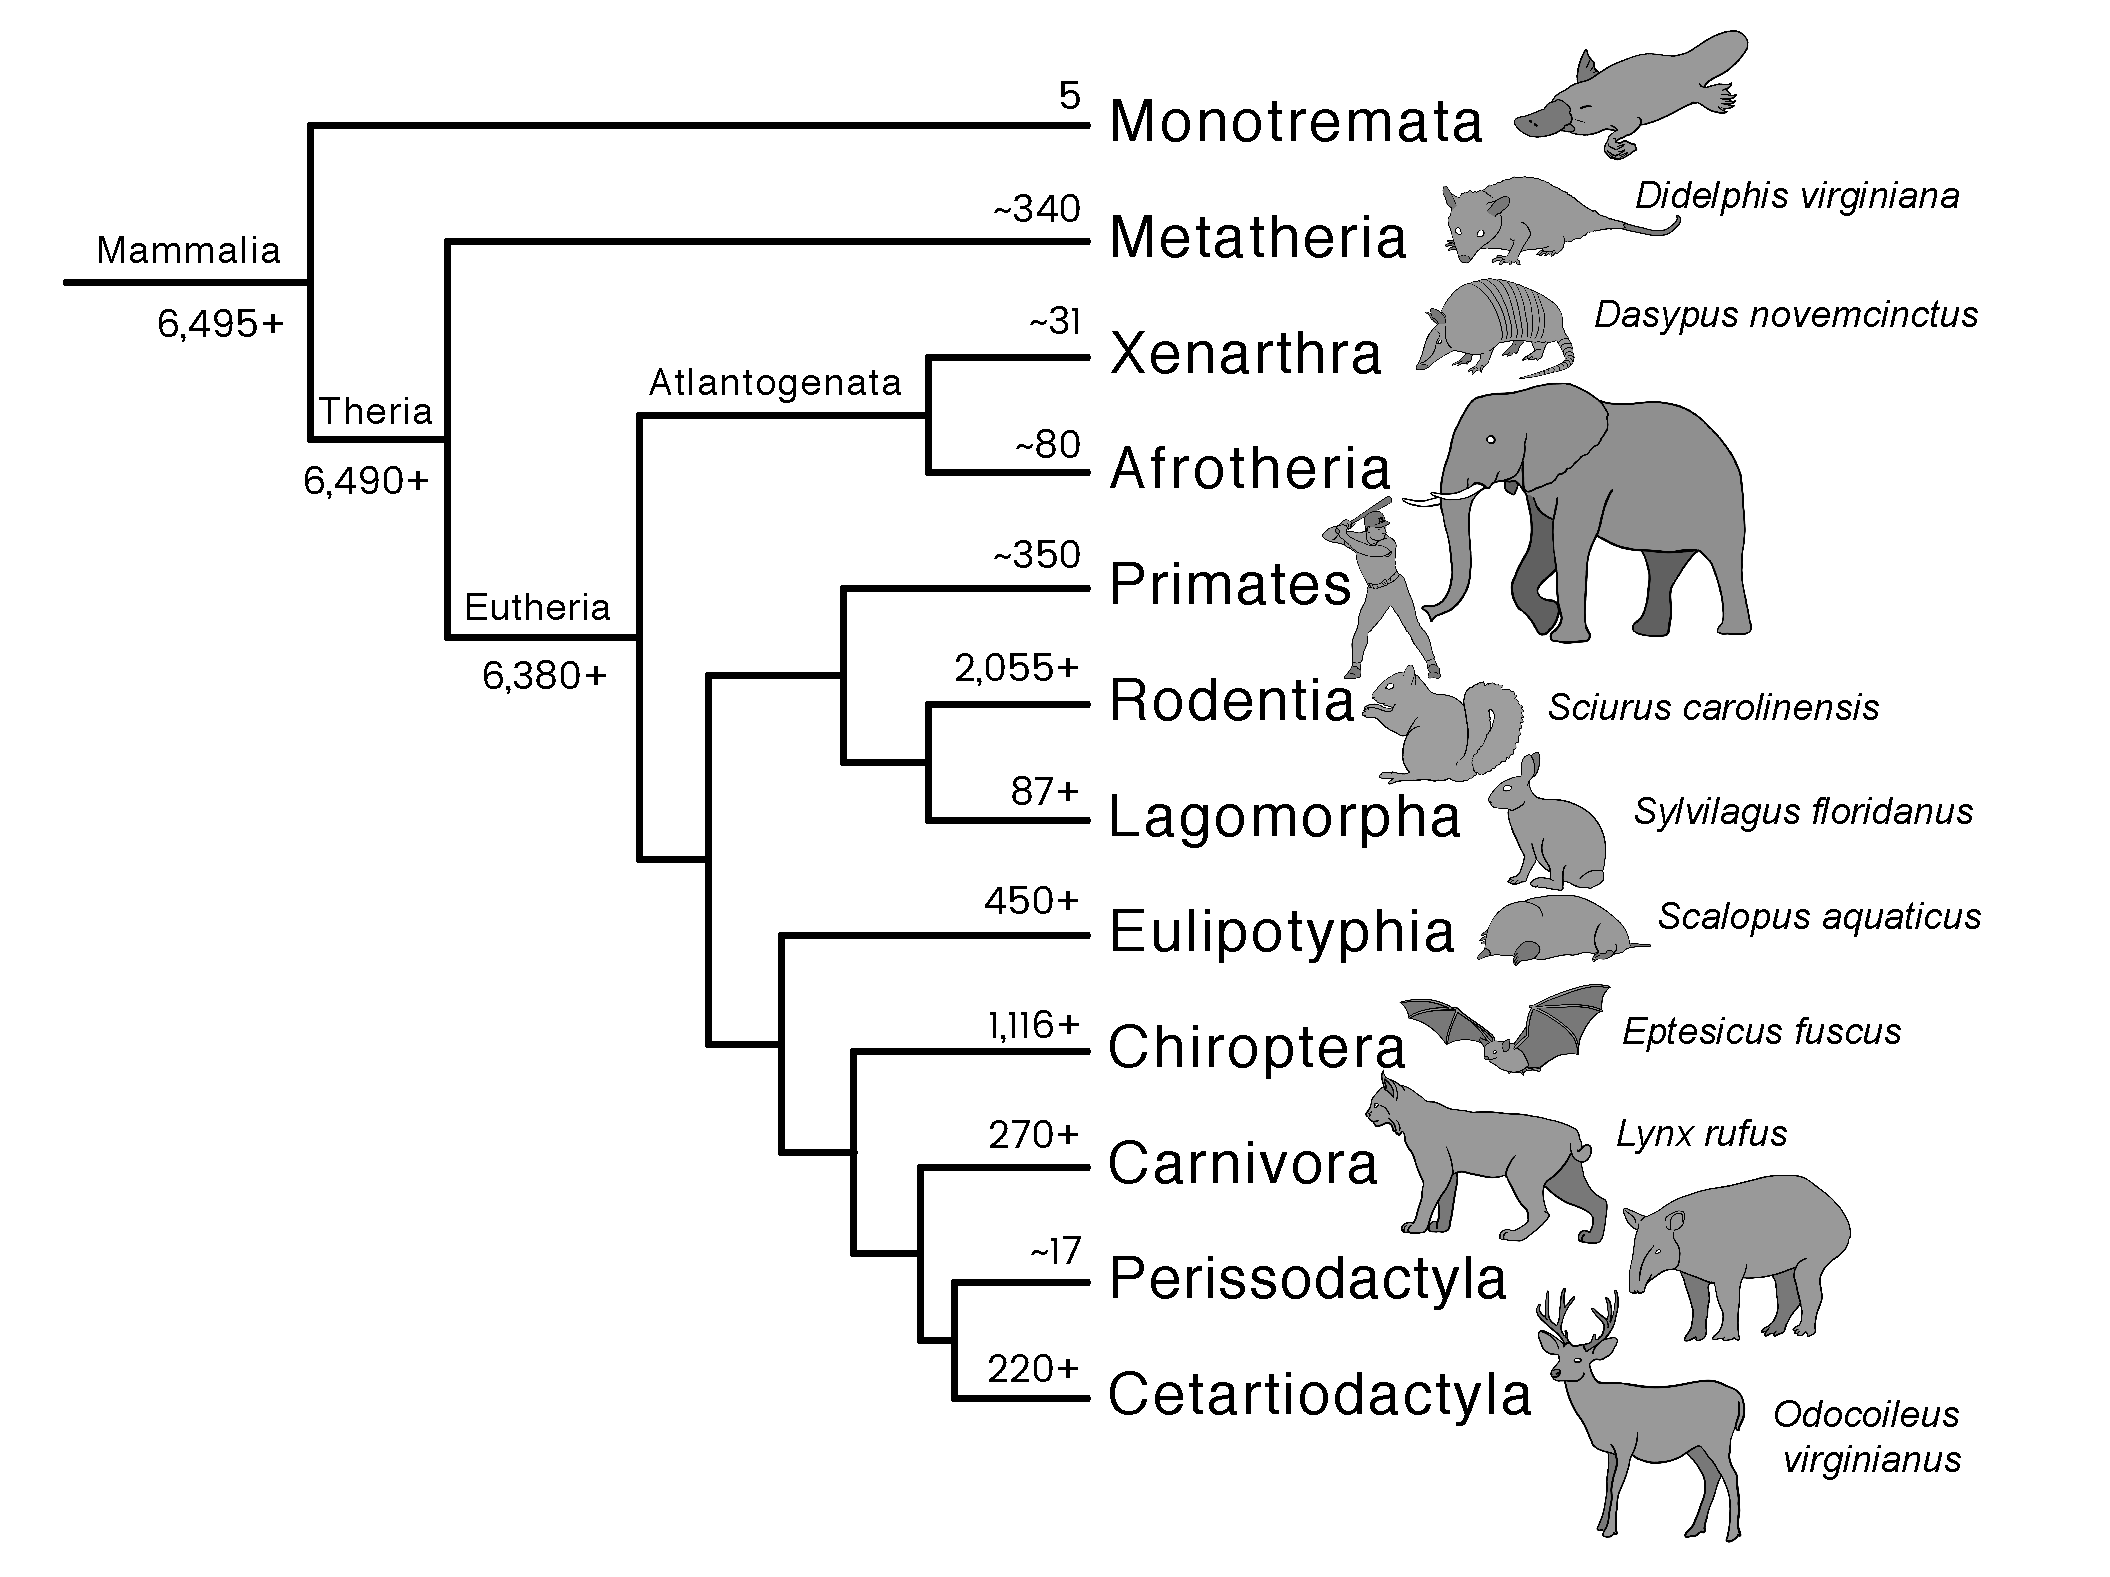
\includegraphics[scale=0.4]{Mammalia_tre.pdf}
  \caption{Mammalian Relationships}
  \label{fig:Mammalia}
\end{figure}

\begin{figure}[H]
\centering
  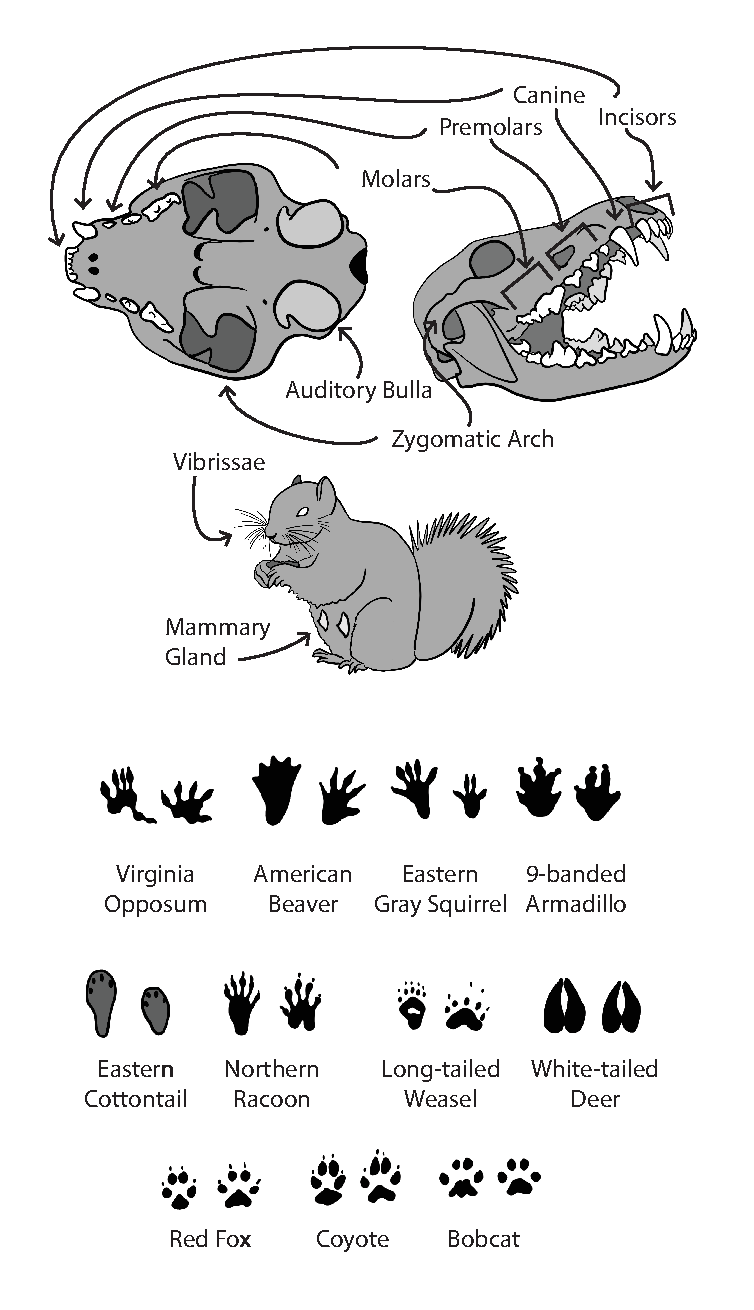
\includegraphics{MammalAnatomy.pdf}
  \caption{Mammalian anatomical terms to know}
  \label{fig:MammalAnatomy}
\end{figure}

\section*{Focal taxonomic groups} ($\star$ groups you need to be able to photo ID and place in a phylogeny. $\mathsection$ denotes species for which you need to know skulls.)
\begin{description}
\item\textbf{Mammalia}
All mammals have hair or fur, mammary glands, unique four chambered hearts, muscular diaphragms, and three ear ossicles.

\begin{itemize}
  \item{\textbf{Monotremata} (monotremes)} \\ Lay eggs and have only a single urogenital opening (cloaca)
  \begin{itemize}
    \item{\textbf{\textit{Ornithorhynchus anatinus}} (duck-billed platypus)$\star$} \\ Have long leathery snout shaped like bill of a duck (used for electrosensory and tactile foraging). Venemous spur on hind foot. Single urogenital opening  (cloaca).
    \item Family {\textbf{TACHYGLOSSIDAE} (echidna)} \\ Have spines over most of body, long slender snout. Single urogenital opening (cloaca). skull: Elongate, rounded snout; laterally bulging brain case. Palate extends backwards to the level of the ears.
  \end{itemize}
  \item{\textbf{Metatheria} (marsupials)} \\ Bony ectotypmanic bulla encasing the middle ear; thick coarse fur, enlarged hind legs, muscular tail, well developed pouch in females (for housing underdeveloped fetus [joey] post birth)
  \begin{itemize}
    \item{\textbf{\textit{Macropus}} (kangaroos and wallabies)} \\ thick coarse fur, enlarged hind legs, muscular tail, well developed pouch in females.
    \item{\textbf{\textit{Didelphis virginiana}} (Virginia opossum)$\star$ $\mathsection$} \\ white face, naked prehensile tail, whitish gray to black fur, well developed pouch in females, highest number of teeth among North American land mammals, large zygomatic arch, strong saggital crest, small braincase. Incomplete auditory bulla. 
      \end{itemize}      
  \item{\textbf{Eutheria} (placental mammals and ancestors)} \\ Bony ectotypmanic bulla encasing the middle ear; an enlarged malleolus ("little hammer") at the bottom of the tibia, the larger of the two shin bones; the joint between the first metatarsal bone and the entocuneiform bone (the outermost of the three cuneiform bones) in the foot is offset farther back than the joint between the second metatarsal and middle cuneiform bones—in metatherians these joints are level with each other.
  \begin{itemize}
    \item{\textbf{Xenarthra} (armadillos, anteaters, and sloths)} \\ additional (xenarthrous) joints of lumbar vertebrae; fusion of the ischium to the anterior caudal vertebrae; a secondary scapular spine; extensive retia mirabile in the limbs; paired postrenal venae cavae; and ossified sternal ribs. Their well-developed claws are used for digging, clinging to tree branches, and defense.
    \begin{itemize}
      \item{\textbf{\textit{Dasypus novemcinctus}} (nine-banded armadillo)$\star$ $\mathsection$} \\ armor of bony dermal plates, long tubular skull, peg-like teeth.
      \item{\textbf{\textit{Myrmecophaga tridactyla}} (giant Anteater)} \\ long tubular head, bushy tail, skull (longer than armadillo), no teeth.
    \end{itemize}
    \item{\textbf{Afrotheria} (enrecs, aardvarks, hyraxes, elephants, and sea cows)} \\ 8 lumbar vertebrae, four allantoic vessel chambers, and the snout is unusually long and mobile in several Afrotherian species (although this may not be a trait shared by ancestry).
    \begin{itemize}
      \item{\textbf{\textit{Trichechus manatus}} (West Indian manatee)$\star$ $\mathsection$} \\ found in warm coastal waters, slow moving aquatic herbivore, continuous teeth replacement from behind, skull lacks sagital crest.
    \end{itemize}
    \item{\textbf{Eulipotyphla} (hedgehogs, shrews, and moles)} \\ small animals with long narrow pointed and usually mobile snouts. They feed on invertebrates, insects and earthworms, and vegetable matter. Small skulls with no distinct canine teeth. Their dental formulae are variable and adapted to hold and crush invertebrates.
    \begin{itemize}
      \item{\textbf{\textit{Scalopus aquaticus}} (eastern mole)$\star$ $\mathsection$} \\ similar to shrew in general appearance, but with large forelimbs for digging and teeth uniform light (not dark at tips).
    \end{itemize}  
    \item{\textbf{Chiroptera} (bats)} \\ Have wings, premolars and molars dissected for slicing invertebrates or fruit. Most insectivorous bats have a divided premaxillae, giving the front of the skull the appearance of horizontal movablejaws.
    \begin{itemize}
      \item{\textbf{\textit{Eptesicus fuscus}} (big brown bat)$\star$ $\mathsection$} \\ dark brown fur, black membranes, blunt tragus (a fleshy, finger-like projection coveringthe entrance to the ear), U-shaped gap between incisors.

    \end{itemize}
    \item{\textbf{Carnivora} (cats, hyenas, dogs, seals, and bears)} \\ Have one pair of premolars and molars (carnassials) enlarged for slicing meat, No toothless space between cheek teeth and front teeth.
    \begin{itemize}
      \item{\textbf{\textit{Lynx rufus}} (bobcat)$\star$ $\mathsection$} \\ reddish tan fur with black spots, short tail with black top, skull more compressed front toback, more rounded than other carnivore skulls, diastema or “gap” posterior to canineteeth.
      \item{\textbf{\textit{Urocyon cinereoargenteus}} (gray fox)} \\ black-tipped tail, black "racing stripe" down back, cat-like face, Lower edge of ramus with distinct step , or break, just in front of angle. Shorter snout than red fox. U-shaped temporal lines (vs V-shaped temporal lines in red fox) 
      \item{\textbf{\textit{Procyon lotor}} (northern raccoon)$\star$ $\mathsection$} \\ black mask, ringed tail. Their forepaws are unusually dextrous and sensitive and resemble slendor human hands but come equipped with 20 non-retractable sharp claws. The dental formula is incisors 3/3, canines 1/1, premolars 3-4/3-4, molars 2/2-3 = 36-42 teeth. Their skulls are thick and heavy and have relatively short rostrums (shorter than canids, longer than felids). Coronoid process higher than condyles; coronoid process concave on posterior side
      \item{\textbf{\textit{Lontra canadensis}} (North American river otter)$\star$ $\mathsection$} \\ dark brown coarse upper fur, silvery fur below, thick tail, webbed feet, skull dorso-ventrally compressed, palate extends beyond tooth row.
    \end{itemize}
    \item{\textbf{Perissodactyla} (horses, zebras, rhinos, tapirs)} \\ Odd toed, no canine teeth
    \item{\textbf{Cetartiodactyla} (deer, pigs, hippos, camels, cows, antelopes, and whales)} \\ Even toed, “cloven hooved”
    \begin{itemize}
      \item{\textbf{\textit{Odocoileus virginianus}} (white-tailed deer)} \\ No incisors, lacrimal bone contacts nasal bone, shallow lacrimal pit, fenestrations = latice-like openings on rostrum of skull, short nasal bones, no upper incisors or canines. * mount and skull
      \item{\textbf{\textit{Bison bison}} (American bison)$\star$ $\mathsection$} \\ body dark brown all over, hump over shoulders, massive head, horns in both sexes, once highly abundant in North America.
      \item{\textbf{\textit{Tursiops truncatus}} (bottlenose dolphin)$\star$ $\mathsection$} \\ thecodont and homodont dentition, large cranium, external nares located medial-dorsally, gray swash on side.
    \end{itemize}  
    \item{\textbf{Primates}} \\ Specialized auditory bulla known as petrosal bulla (bulla fused to petrosal bone) to protect middle ear. 
    \item{\textbf{Rodentia} (rodents)} \\ Have one pair elongate and ever-growing incisors, distinct space between incisors and cheek teeth
    \begin{itemize}
      \item{\textbf{\textit{Sciurus carolinensis}} (eastern gray squirrel)$\star$ $\mathsection$} \\ Coronoid process short, gray fur, very bushy tail, the “common” squirrel; skull with extra peg-like tooth inmolariform tooth row. 
      \item{\textbf{\textit{Glaucomys volans}} (southern flying squirrel)$\star$} \\ Coronoid process short, very soft fur, gray brown above white below, loose skin along side (patagium) forms gliding surface, strictly nocturnal. 
      \item{\textbf{\textit{Castor canadensis}} (American beaver)$\star$ $\mathsection$} \\ very large size, thick brown fur, flattened hairless scaly tail, very large orange incisors, distinct bump on lower end of remus beneath cheek teeth.
    \end{itemize}
    \item{\textbf{Lagomorpha} (rabbits, hares, and pika)} \\ Have two pairs of incisors, one pair of evergrowing and elongate the second pair small and peg-like, fenestrations = latice-like openings on rostrum of skull
    \begin{itemize}
      \item{\textbf{\textit{Sylvilagus floridanus}} (eastern cottontail)$\star$ $\mathsection$} \\ mixed brown and buff fur above, noticeable rusty spot on nape, whitish feet andunderside.
    \end{itemize}
  \end{itemize}
\end{itemize}
\end{description}

\end{document}
